% ==============================================================================
%\chapter{White Rabbit Network Topology and Dimensions}
\section{White Rabbit Network Topology and Dimensions}  
% ==============================================================================



The features of WR network comes at a price of topology
limitations. A proper operation of WR Network is based on a careful design of
its topology which must fulfil requirements presented in this chapter. Within
the limitations of presented requirements, the topology can implement different
levels of redundancy to provide reliability suited to user's needs. Example
topologies are presented.

\subsection{WR Network Dimension}

White Rabbit is a deterministic network. In terms of determinism,
network dimension is understood as the number of hops (switches) and the length
of physical connection (fibre or copper) that an Ethernet frame needs to
traverse on the longest possible path in the network. It is important to notice
that the distinction between Control Data (i.e. \ControlMessage s) and Standard
Data does apply. For a \ControlMessage s, the path is always from Data Master to
a node. For a non-\ControlMessage s, the path can be between any two nodes.
Since the timing requirements (i.e. \GW) concern Control Data, the following
analysis will take into account only Control Data.

In terms of network usage, network dimension is understood as the
possible number of end devices which can be connected. In terms of
network costs, network dimension is understood as the number of switches and
links needed to connect required number of end devices. There is no direct
translation between the number of switches (hops) in the network and the number
of end devices. This relationship depends on the network topology. However, the
possible range of the numbers can be calculated. To do that, various levels of
network topology's redundancy are considered (the topologies are tree
topologies):
\begin{itemize}
  \item \textbf{no-redundancy} - each switch is connected to 16 switches
or nodes by its downlinks and one switch/node by its uplink (one uplink is
free). 
  \item \textbf{double redundancy} - each switch is connected to two
separate switches/nodes by its uplinks and to 16 switches/nodes by its
downlinks. 
  \item \textbf{triple redundancy} - each switch is connected to three separate
switches/nodes by its uplinks \footnote{Hardware-wise possible in V3 Switch} and
to 15 switches/nodes by its downlinks. 

\end{itemize}

In principle, each WR Switch has two uplinks and 16 downlinks, however V3 of WR
Switch enables any number of ports to act as uplinks. Uplinks are supposed to
be connected to the source of timing information, i.e. downlinks of White Rabbit
Switch or Node. 

In order to satisfy the requirements (~2000 end devices), 3 or 4 layers of
switches are needed depending on the topology type. The relationship between
number of hops (switches), the length of the link and the Control Message
Delivery Delay can be expressed by equation:
\begin{equation}
	Delay_{CM} = D * delay_{link} + N * delay_{sw} + delay_{n\_tx}
+ delay_{n\_rx} + delay_{enFEC} + delay_{deFEC}
\end{equation}	
where all $delay_{x}$ parameters are given in the column Value Max of the
Table~\ref{tab:CMdelayHP}, the $D$ and $N$ parameters are thelink length in [km]
and number of hops respectively. $Delay_{CM}$ needs to fulfil requirements for
\GranularityWindow ($100\mu s$ for GSI, $1000\mu s$ for CERN).
The relationship between $Delay_{CM}$, $D$ and $N$ is shown in the
Figure~\ref{fig:deliveryDelayChart}.

\begin{center}
	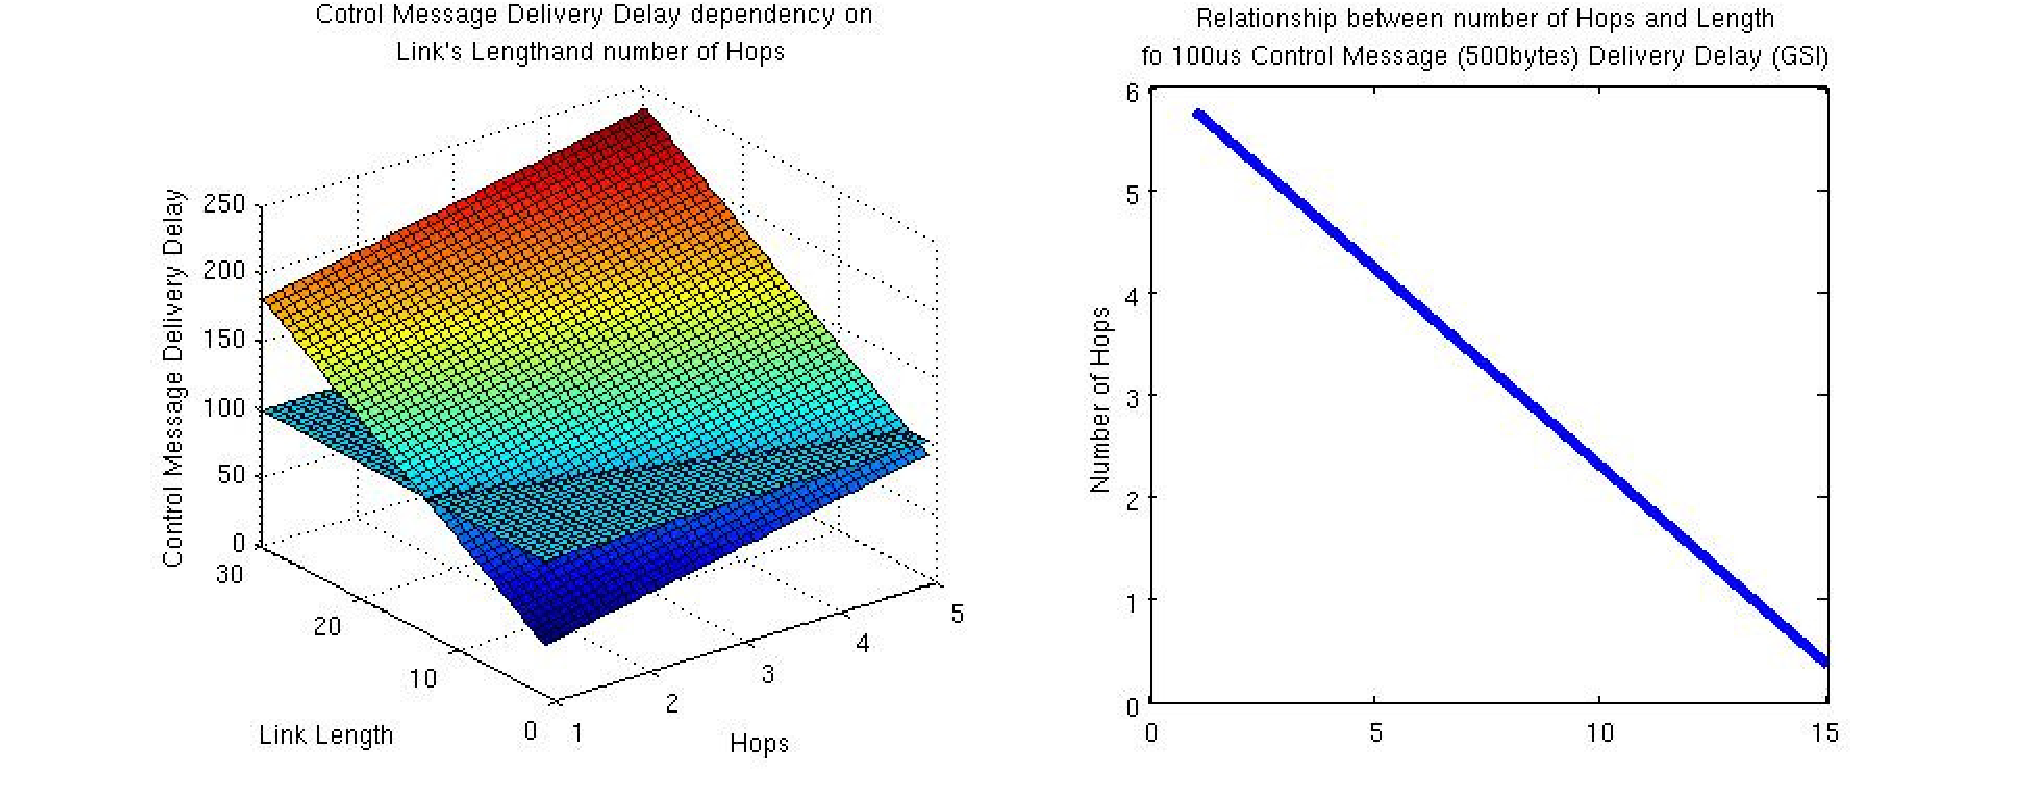
\includegraphics[scale=0.40]{../../../../figures/robustness/deliveryDelayChart.ps}
	\captionof{figure}{The relationship between $Delay_{CM}$, $D$ and $N$.}
	\label{fig:deliveryDelayChart}
\end{center}

As explained in Chapter~\ref{reliabilityOfNetwork}, various topologies of WR
Network are considered to have N-inputs (connections to Data Master) and
N-outputs (connections to nodes), where N is 1 for topology with no redundancy,
2 for double redundancy, 3 for triple redundancy. 

Table~\ref{tab:translation3topologies} shows the number of switches and the
number of their layers required to achieve a given number of end devices (nodes)
for three different topologies.
For example, in order to connect 2000 WR nodes with triple redundancy, WR
Network needs to consists of 4 layers of switches (total of 499 WR switches),
for non-redundant topology 3 layers of 273 WR Switches are needed. 

However, as described in Chapter~\ref{jitterDeterminismNetworkDimention}, it is
desirable to have at most 3 layers of switches. Connecting $\approx$ 2000 of
nodes in double- or triple- redundant topology of 3 layers is possible if we
consider the number of network inputs (M) to be greater then network outputs
(N). Table~\ref{2000nodes3topologies} compares topologies with M-inputs and
N-outputs ($M>M$) which enable to connect 2000 nodes.

\begin{table}[ht]
\caption{Translation between number of switches, number of layers of switch 
(hops), type of redundancy and number of end devices(nodes) for
N-inputs/N-outputs network.} 
\centering 
\begin{tabular}{| p{1.9cm} | p{2.7cm} | p{2.7cm} | p{2.5cm} |}       
\hline
\textbf{Switch Layer Number}& \multicolumn{3}{|c|}{\textbf{Number of
Switches/end devices}}  \\
      & triple redundancy & double redundancy & no redundancy   \\ \hline
0     & 3                 & 2                 & 1                  \\ \hline
1     & 16                & 16                & 16                \\ \hline
2     & 80                & 128               & 256               \\ \hline
3     & 400               & 1024              & 4096             \\ \hline
4     & 2 000             & 8 192             & 65024          \\ \hline
5     & 10 000            & 16 384            & 1040384        \\ \hline
\end{tabular}
\label{tab:translation3topologies}
\end{table}

\begin{table}[ht]
\caption{Number of WR Switches in a network with ~2000 nodes for different
topologies of 3-switch-layers.} 
\centering 
\begin{tabular}{| p{6cm} | p{2.0cm} | p{2.0cm} | p{2.0cm} | }       
\hline
 & \textbf{triple redundancy}&\textbf{double redundancy}  &\textbf{no
redundancy} \\
      &  &  &    \\ \hline
Number of Network inputs 
(connections to Data Master) & 15& 4           & 1               \\ \hline
Number of End devices  & 2000    & 2048        & 2048            \\ \hline
Total number of Switches     & 495     & 292         & 137                 \\
\hline
Number of Network outpus 
(connections to a node) & 3        & 2           & 1               \\ \hline

\end{tabular}
\label{tab:2000nodes3topologies}
\end{table}

\newpage

\subsection{WR Network Topology Requirements} 

A White Rabbit Network:
\begin{itemize}
  \item shall have tree/star topology;

  \item shall include the following components :
  \begin{itemize}
       \item  Data Master WR Node(s) - source of Control Information,
       \item  Receiving WR Node(s) - recipients of Control and Timing
	      Information,
       \item  Data Timing WR Node(s) or Switch(s) - source of Timing
	      Information (connected to GPS receiver)
       \item  WR Switch
  \end{itemize}

  \item might include non-WR devices which shall be connected to downlinks of a
	  WR Switch:
  \begin{itemize}
       \item  non-WR Receiving Node(s),
       \item  non-WR Switch(es),
  \end{itemize}

  \item shall fulfil the following requirements concerning WR Nodes connection:
  \begin{itemize}
       \item  Data Master WR Node - connected to RSTP Root Switch or RSTP
	      Backup Root Switch,
       \item  Data Timing WR Node - connected to uplink of a WR Switch,
       \item  Receiving WR Node - connected to downlink of a WR Switch;
  \end{itemize}
 
 \item shall be configured in such way, that Rapids Spannig Tree Algorithm
	elects as Root Switch a WR Switch connected to Primary Data Master WR
	Node; 

  \item shall include WR Switches whose:
  \begin{itemize}
        \item  at least single uplink is connected,
        \item  uplink(s) is connected to Data Master WR Node, Timing
		Master WR Nodes or downlinks of WR Switches which are at the
		same or higher topology layer,
        \item  downlinks are connected to WR Nodes (excluding Data Master and
		Timing Master), uplinks of WR Switches, or non-WR devices.
  \end{itemize}

  \item shall not have ring topology; 

  \item might have one or two Data Master WR Nodes. If two Data Masters are
	present, only single Data Master can be active at a time. We call an
	active Data Master: Primary Data Master, the other is called Backup Data
	Master, see Figure~\ref{fig:wrRSTPtopologies}. Backup Data Master:
  \begin{itemize}
        \item  might be connected to the same WR Switch(s) as Primary Data
	       Master,
        \item  might be connected to a different WR Switch then Primary Data
	       Master, in such case the switch is called Backup Root WR Switch
	       and it needs to be connected to RSTP Root Switch with two
	       links;
  \end{itemize}

  \item including Backup RSTP Root Switch shall fulfil the following
	requirements:
  \begin{itemize}
        \item  (1)Backup RSTP Root and RSTP Root Switches shall be connected
	       by two links (uplink-downlink), if Backup Root Switch is
	       connected to only to Backup Data Master only, or
	\item  (2)Backup RSTP Root shall be connected directly to Primary Data
		Master,
        \item  in both cases (1) \& (2), the configuration shall ensures that
		Backup Root Switch is the second best for RSTP Root,
  \end{itemize}
	
  \item shall distinguish 3 layers (Figure~\ref{fig:WRtopology}):
  \begin{itemize}
        \item Core Layer: Primary Root Switch and (optionally) Backup Root
	      Switch
        \item Distribution Layer: WR Switches connected to Core Layer by
	      uplinks, uplinks of Distribution Layer Switches shall be
	      connected to Access or Distribution Layer Switches only, no WR
	      Nodes are allowed.
        \item Access Layer: Switches connected by uplinks to Distribution
	      Layer, by downlinks to Nodes.
  \end{itemize}

  \item shall preferably have all the Receiving Nodes connected only to the
	lowest layer of WR Switches (Access Layer).
  \item must fulfil the following requirement length of data/clock path: 
  \begin{itemize}
        \item we define length of data/clock path as the number of hops from a
	      given WR Switch to Data Master,	
        \item we define primary data/clock path, as the path seen from root
	      port of a given WR Switch,
        \item we define backup data/clock path, as the path seen from backup
	      port of a given WR Switch,
	\item the difference between the length of primary and backup data/clock
	      path shall be not grater then one hop.
  \end{itemize}
 
 \end{itemize}


\begin{center}
	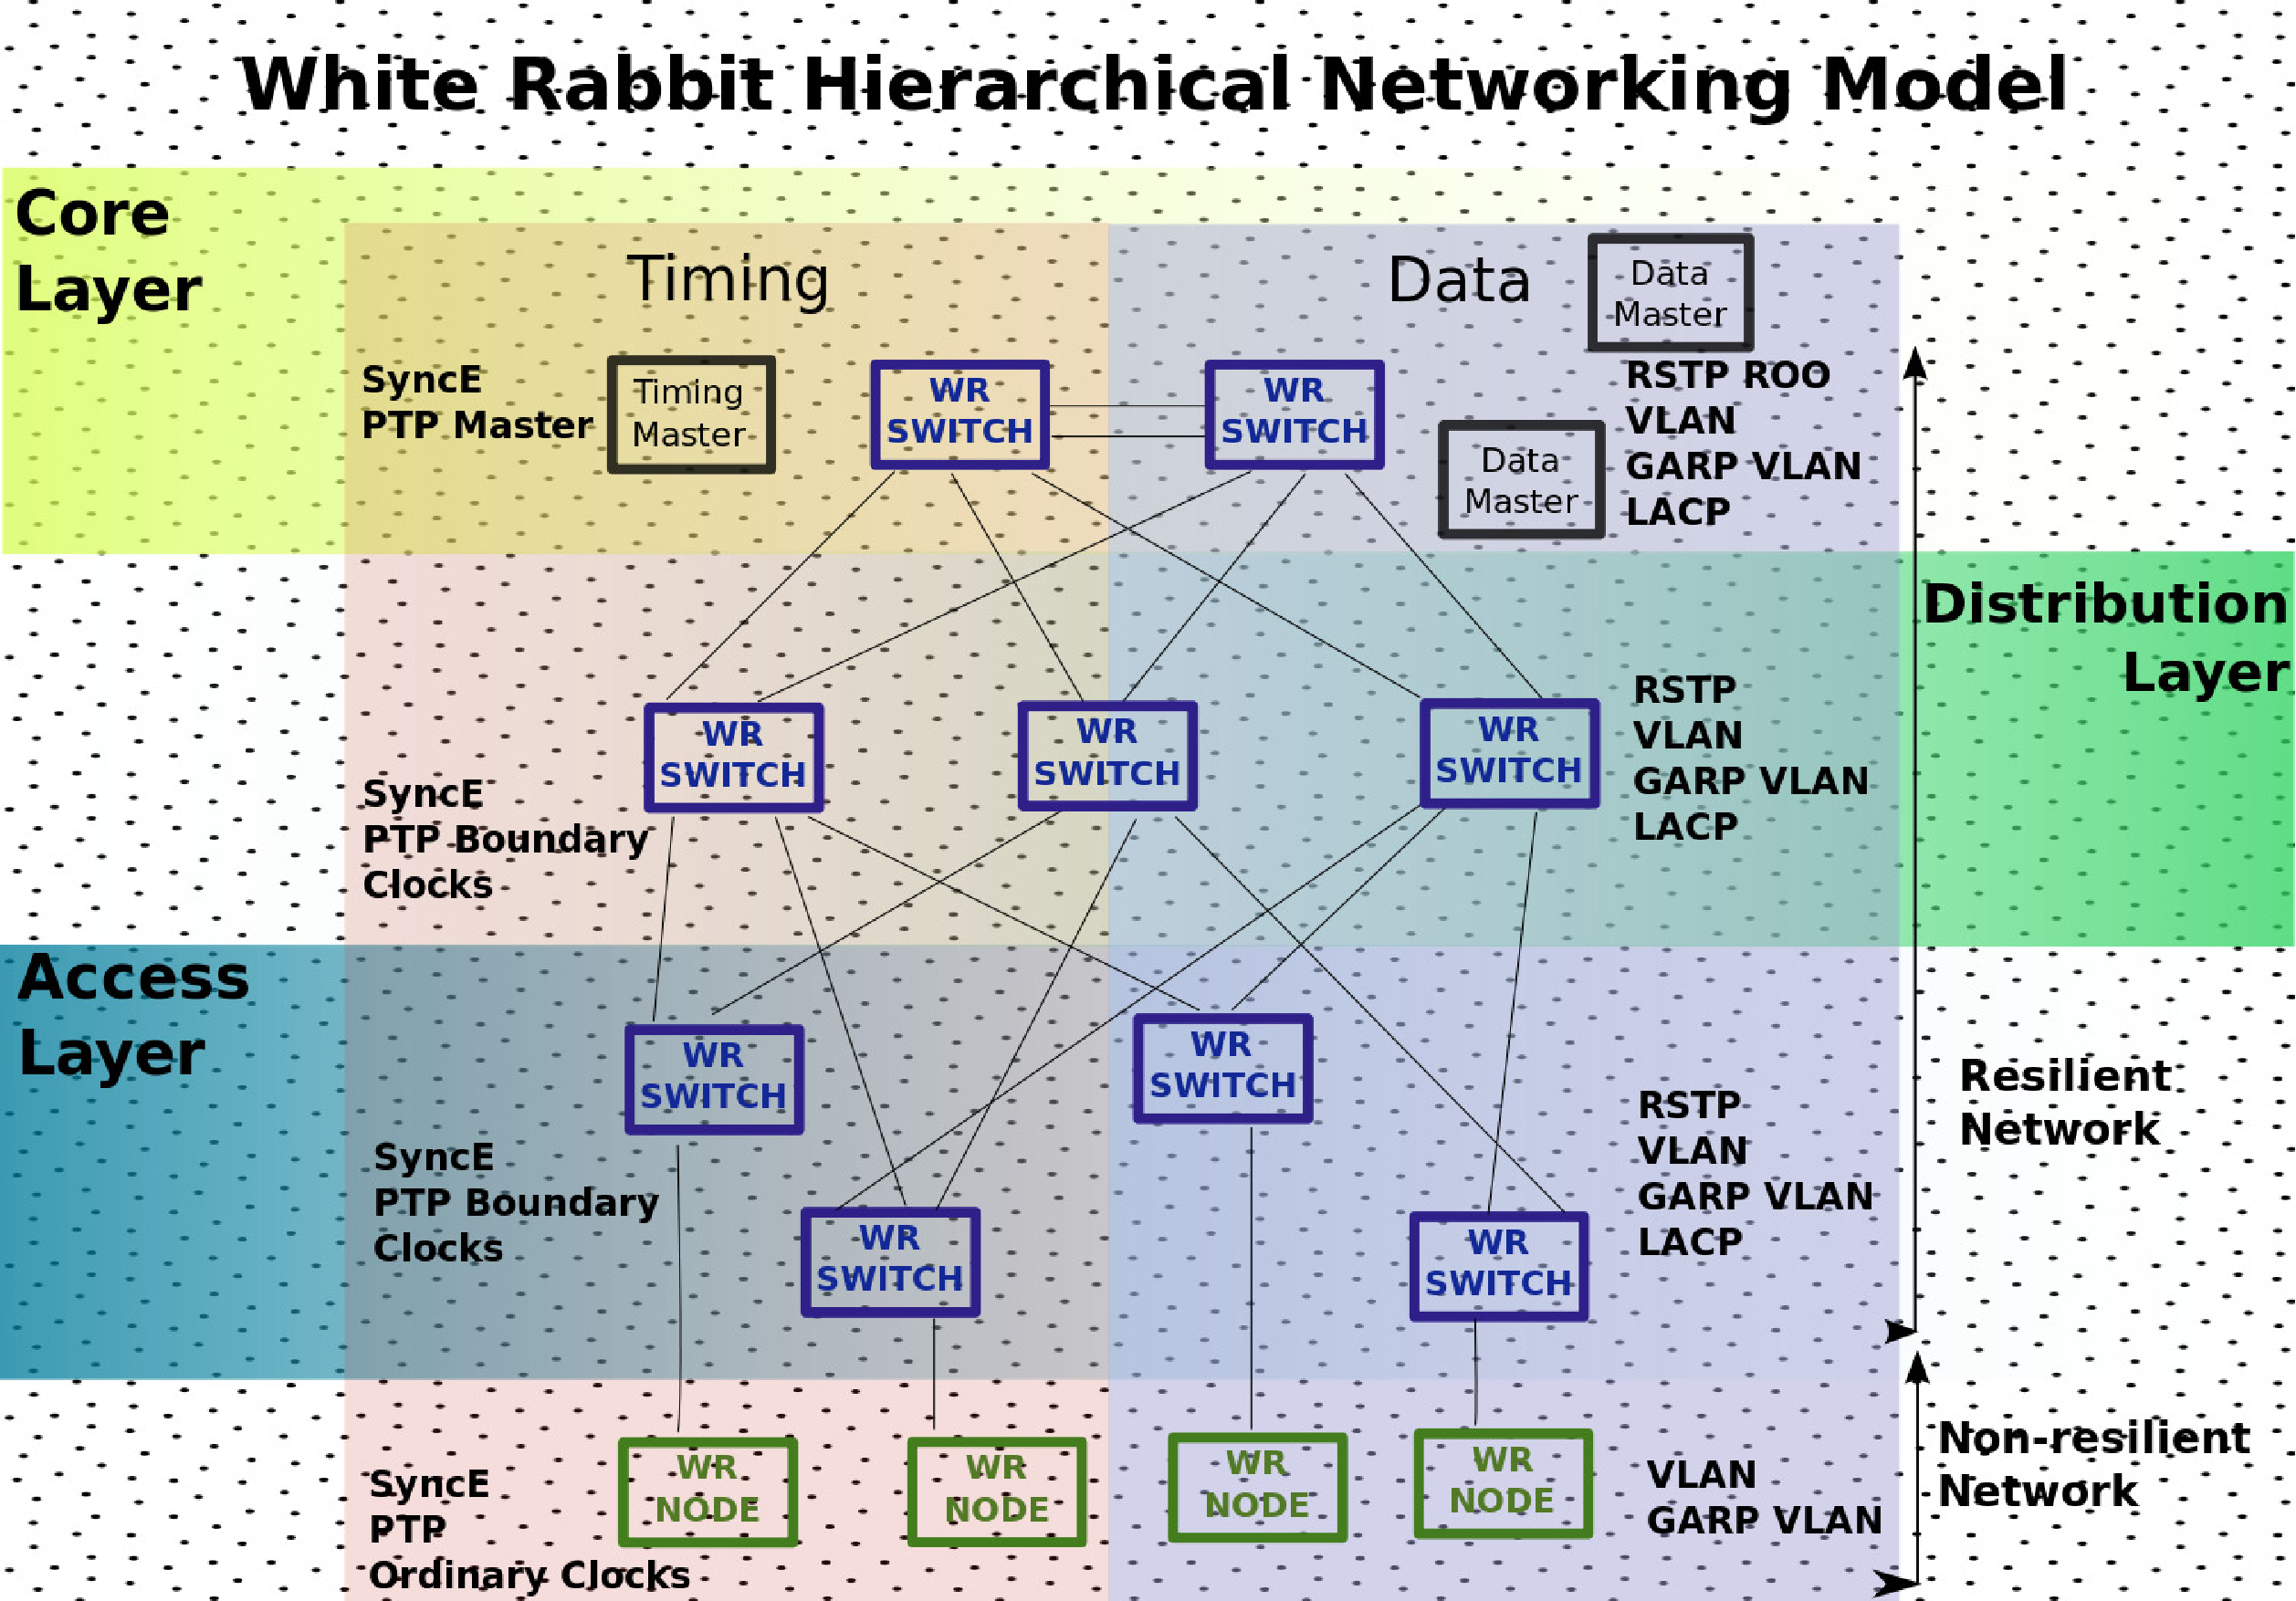
\includegraphics[scale=0.35]{../../../../figures/network/hierarchy2.ps}
	\captionof{figure}{Example WR topology.}
	\label{fig:WRtopology}
\end{center}

\section{Reliability of WR Network}
\label{reliabilityOfNetwork}

The following chapters use the terms :
\begin{itemize}
  \item Mean Time Between Failure (MTBF) of a component/entire network (the
bigger the better) and
  \item probability ($P_f$) of failure of a component/entire network (the
smaller the better)
\end{itemize}
to measure reliability. Convention presented in \cite{DesigningLSLANs}
\footnote{The choice of reference might have been unfortunate, it seems that
the book makes too great simplifications, this needs to be verified and more
detailed studies/calculations performed for the next release of the doc.} is
used to define relation between these two terms (equation \ref{eq:mtbf}). A
detailed
explanation of MTBF and $P_f$ can be found in Appendix~\ref{appA}. 
	\begin{equation}
        \label{eq:mtbf}
		P_f= \frac{1 [day]}{2*MTBF [h]}  
	\end{equation}

A WR Network is considered functional, if all its Receiving Nodes are provided
with Control and Timing Information - there is a Data and Timing Path from Data
Master to each Receiving WR Node. 

Data Master WR Node and Receiving WR Node can be connected to the network of
interconnected WR Switches in several ways, see 
Figure~\ref{fig:topologyConsideration}. For the comparison of different
network topologies, we consider reliability of a network of WR Switches
(excluding Data Master and Receiving Node) with N inputs and N
outputs, as depicted in Figure~\ref{fig:topologyConsideration}: R0. The
number of inputs/outputs (N) reflects the level of redundancy. This means that a
network with triple redundancy is considered to have three inputs and three
outputs. The inputs are provided with exactly the same data. A valid data on
one of the outputs is considered sufficient for the network to be functional.
The reasons to do so are given below.
\begin{itemize}
  \item It allows to abstract from the way Data Master and Receiving Nodes are
connected.
  \item Single input/output to/from the network enforces single point of
failure in the network, this makes the network less reliable then the
reliability of this component (switch, link) which is the single point of
failure.
  \item Introducing redundancy in a network is reasonable, only if the
redundant network's reliability is similar to the reliability of Receiving WR
Node (and non-redundant Data Master). If the reliability of single Data Master
is a few orders of magnitude less then the reliability of redundant network,
introducing redundancy to a network is simply a waste of money.
\end{itemize}

However, in order to reach the number of $\approx$ 2000 nodes with only 3
layers of switches, it might be needed to provide greater number of inputs to
the WR Network (connetions with Data Master) then outputs, see
Figure~\ref{fig:topologyConsideration}: R1.

The values of MTBFs of components used in the calculations are just examples,
the real MTBF of WR Switch is not known. 200 000 hours is an average MTBF for
Cisco Switches. Two other values for WR Switch are used in the calculations to
represent very reliable switch (1 000 000 hours) and moderately reliable switch
(20 000 hours). 
\begin{table}[ht]
\caption{Component failure-failure probabilities \cite{The All-New Switch Book:
The Complete Guide to LAN Switching Technology}. }
\centering
\begin{tabular}{|c|c|c|c|}          \hline
\textbf{Component}& \textbf{MTBF} & \textbf{Probability} \\
                  &    [h]       &        [\%]   \\ \hline
Copper connection &   1 000 000   &   0.001 2  \\ \hline
Fibre Connection  &   1 000 000   &   0.001 2  \\ \hline
WR Switch (medium reliability)&     200 000   &   0.006 0  \\ \hline
WR Switch (very reliable)     &   1 000 000   &   0.001 2  \\ \hline
WR Switch (low reliability)   &      20 000   &   0.060 0 \\ \hline

\end{tabular}
\label{tab:MTBFandProbabilityOfComponents}
\end{table}


\begin{center}
	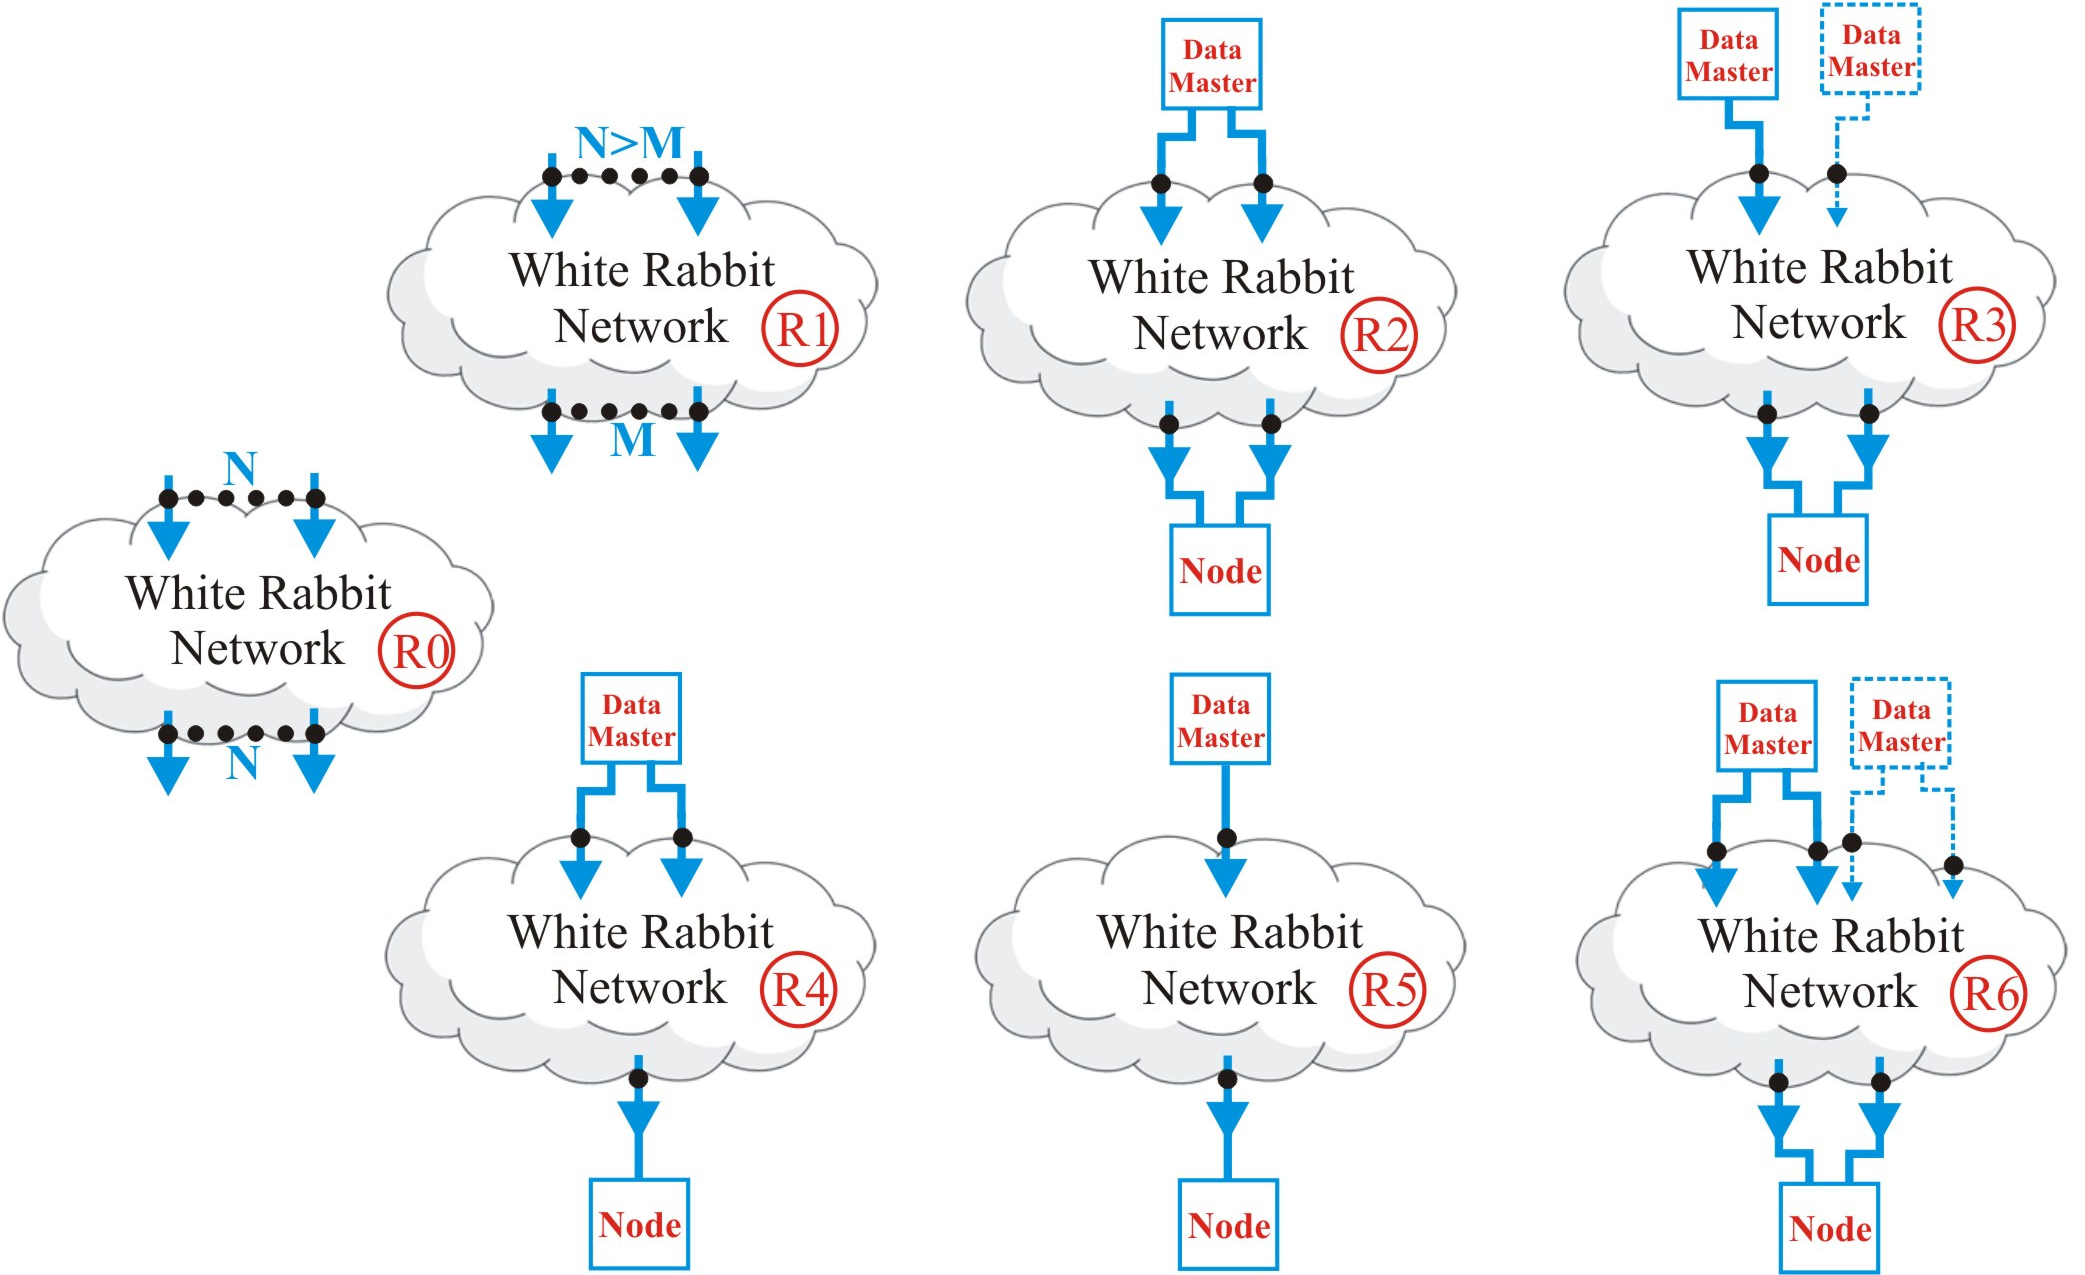
\includegraphics[scale=0.35]{../../../../figures/robustness/topologyConsideration.ps}
	\captionof{figure}{WR Network Connections to Data Master(s) and
Receiving Node.}
	\label{fig:topologyConsideration}
\end{center}

\subsection{WR Network Topology Examples}
\label{WRnetworkTopologyExamples}
Three different topologies with various levels of redundancy are compared
below (Table~\ref{tab:nonRedundantTopology}). As can be seen in
Figure~\ref{fig:threeTopology}, these are the least
optimal (in terms of "number of switches to number of nodes" ratio) topologies
with N inputs/outputs. For each of the topologies, two-terminal
\footnote{Between Data Master and single node.} probability of failure ($P_f$)
and MTBF were calculated using \cite{FaultTree}. 

A number of topologies is possible within the same level of redundancy. A few
example topologes with double redundancy are depicted in
Figure~\ref{fig:fullyRedundantTopologies}.

\begin{table}[ht]
\caption{Comparison of topologies, see Figure~\ref{fig:threeTopology}
for illustration.}
\centering
\begin{tabular}{|p{0.5cm}|p{1cm}|p{1.1cm}|p{1.7cm}|p{1.5cm}|p{1.9cm}|p{1.7cm}
|p{1.9cm}|p{1.7cm}|}        \hline
& \textbf{WRS Number} &
\textbf{Nodes MAX Number} &  
\multicolumn{2}{|p{3cm}|}{\textbf{$MTBF_{Switch}$=    20 000 [h] }} &  
\multicolumn{2}{|p{3cm}|}{\textbf{$MTBF_{Switch}$=   200 000 [h] }} &
\multicolumn{2}{|p{3cm}|}{\textbf{$MTBF_{Switch}$= 1 000 000 [h] }}\\
 & & & $P_f$ & MTBF[h] & $P_f$ & MTBF[h] &
$P_f$   & MTBF[h] \\ \hline
%1   &   3   &  14336  &   r1   &   r2   &   r3   &   r4   &   r5    \\ \hline

T1 &  273 &  4096  
& $ 3.66*10^{-3}$  & $ 6.56*10^{3}$
& $4.32*10^{-4}$  &  $ 5.55*10^{4}$    
& $1.44*10^{-4}$  &  $ 1.66*10^{5}$  \\ \hline

T2 &  146 &  1024  
& $ 1.60*10^{-6}$  &  $ 1.50*10^{7}$
& $ 2.07*10^{-8}$  &  $ 1.16*10^{9}$    
& $ 2.3*10^{-9}$   &  $ 1.04*10^{10}$   \\ \hline

T3 &  90  &  400   
& $ 3.55*10^{-9}$  &  $ 6.76*10^{9}$
& $ 4.71*10^{-12}$ &  $ 5.09*10^{12}$    
& $ 1.24*10^{-13}$ &  $ 1.93*10^{14}$  \\ \hline
\end{tabular}
\label{tab:nonRedundantTopology}
\end{table}


\begin{center}
	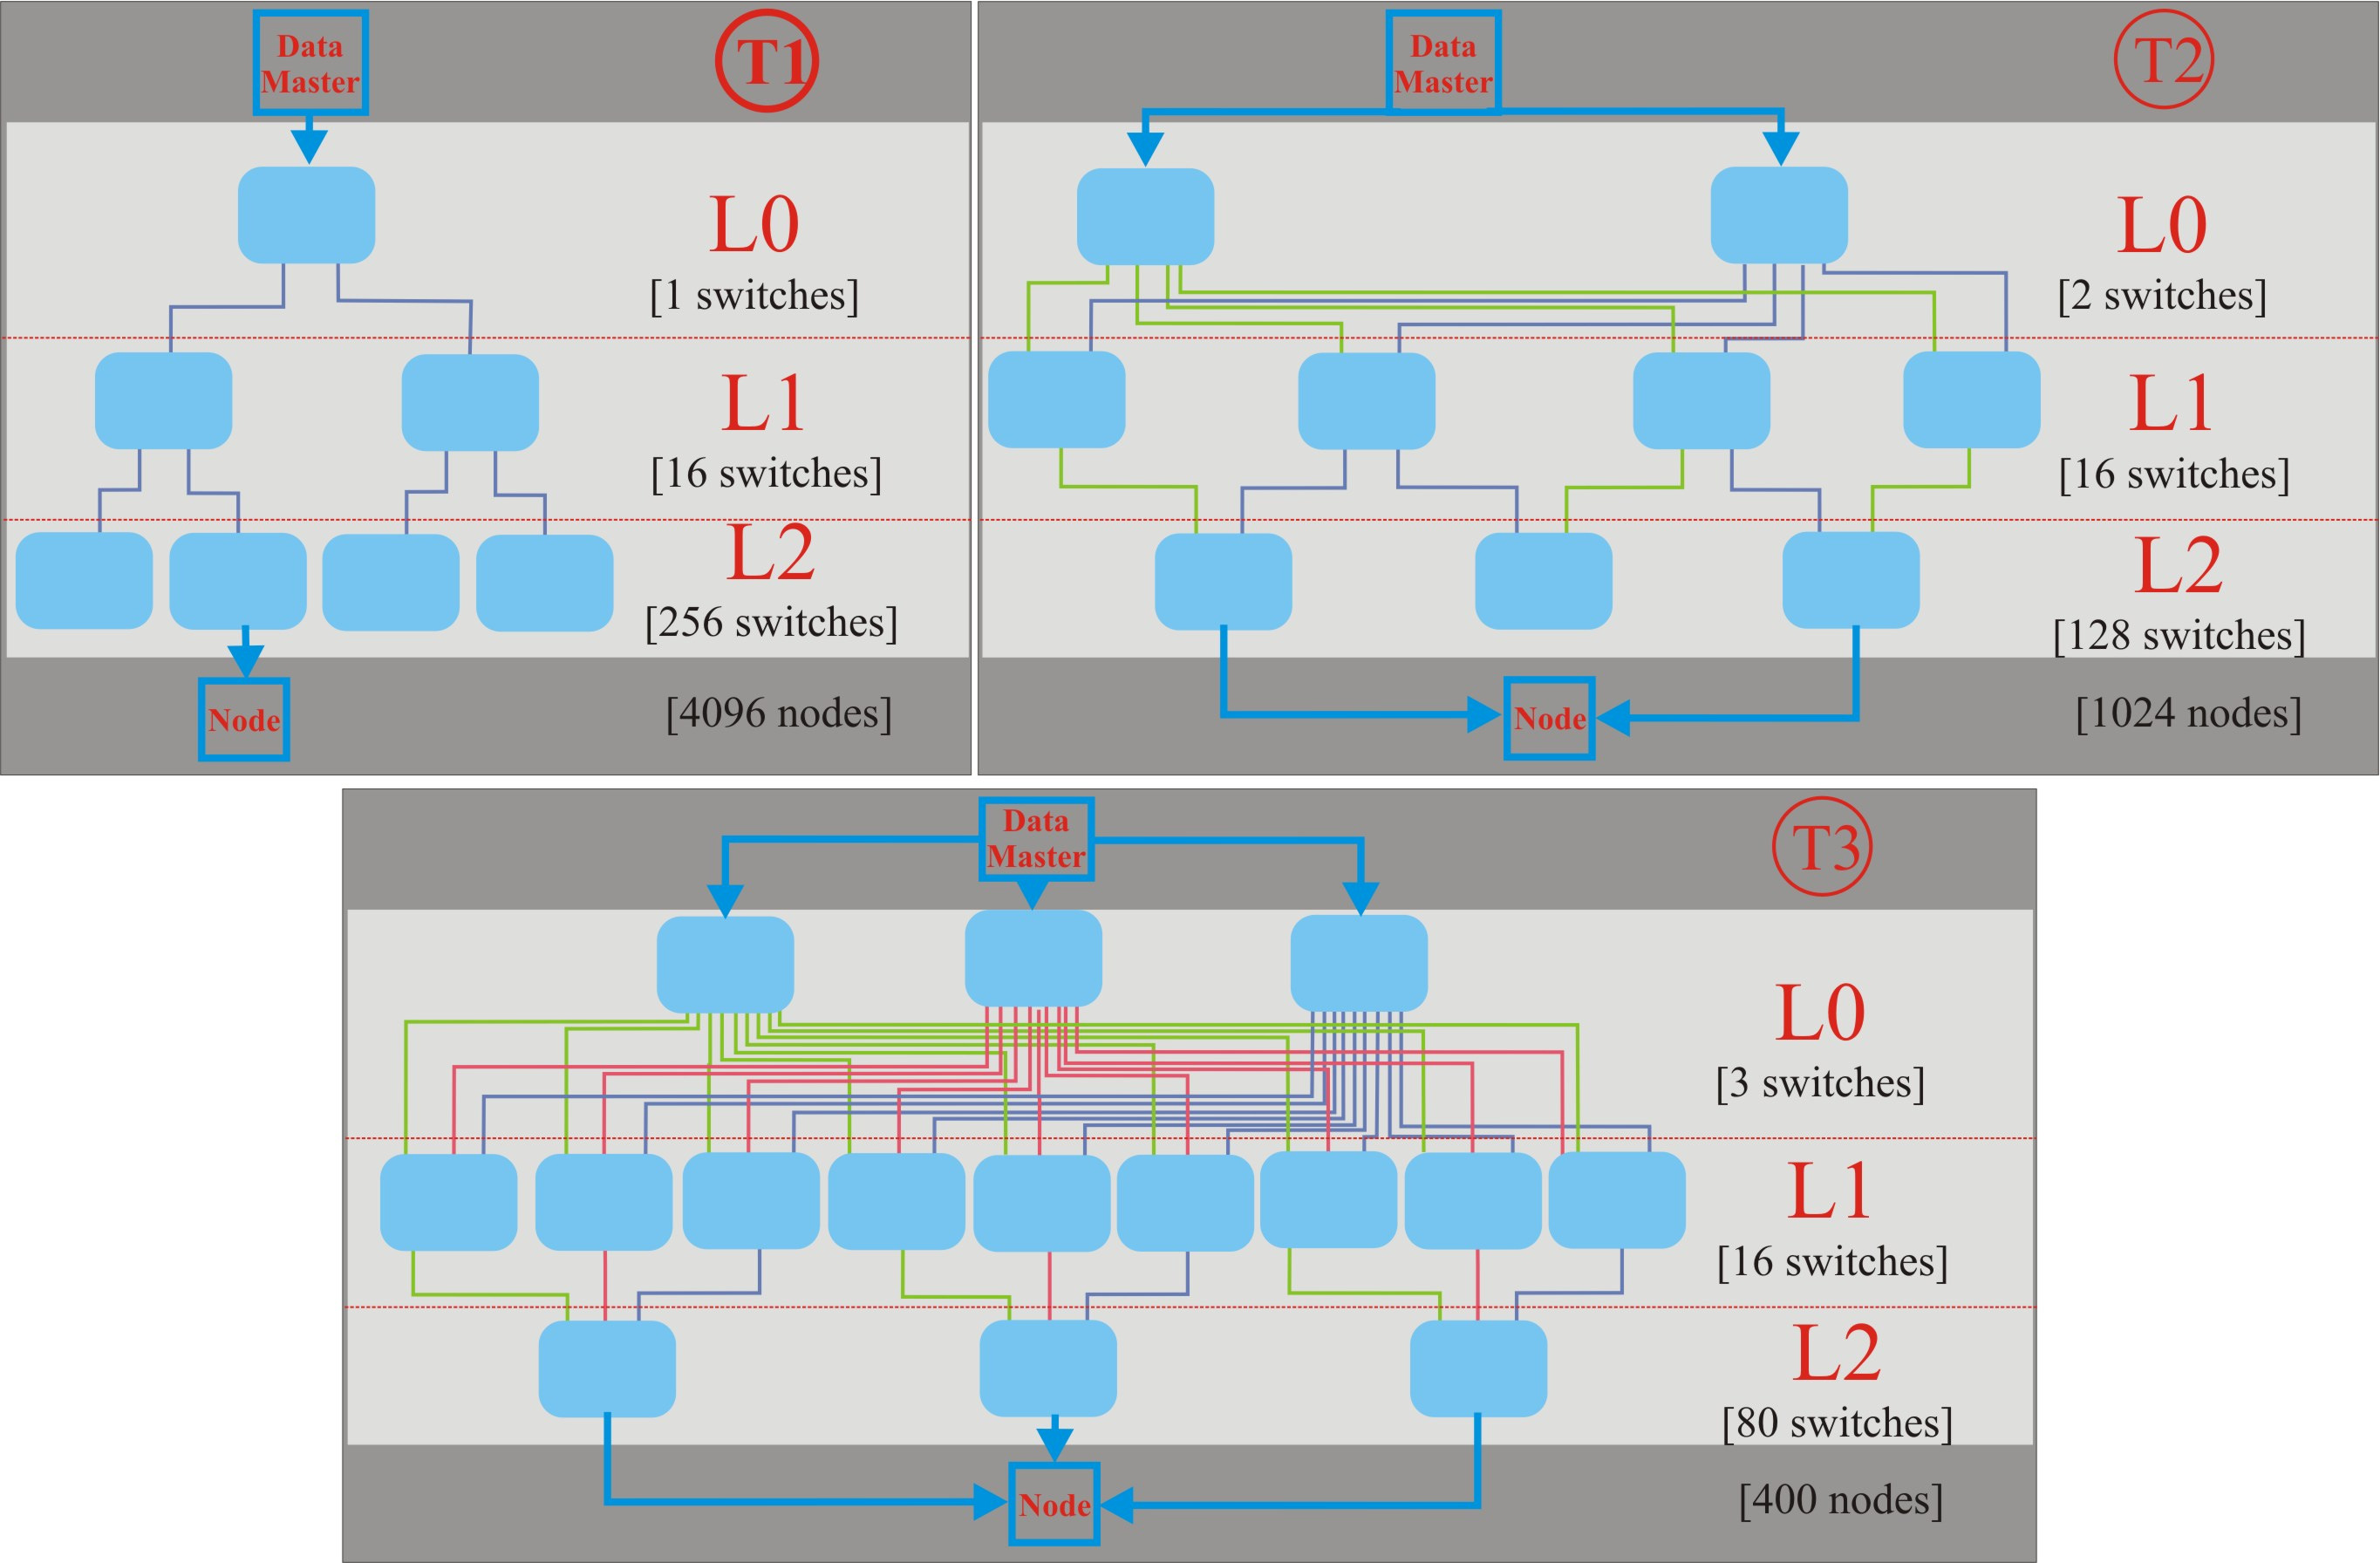
\includegraphics[scale=0.25]{../../../../figures/robustness/threeTopologies.ps}
	\captionof{figure}{Examples of topologies with different level of
redundancy.}
	\label{fig:threeTopology}
\end{center}

\begin{center}
	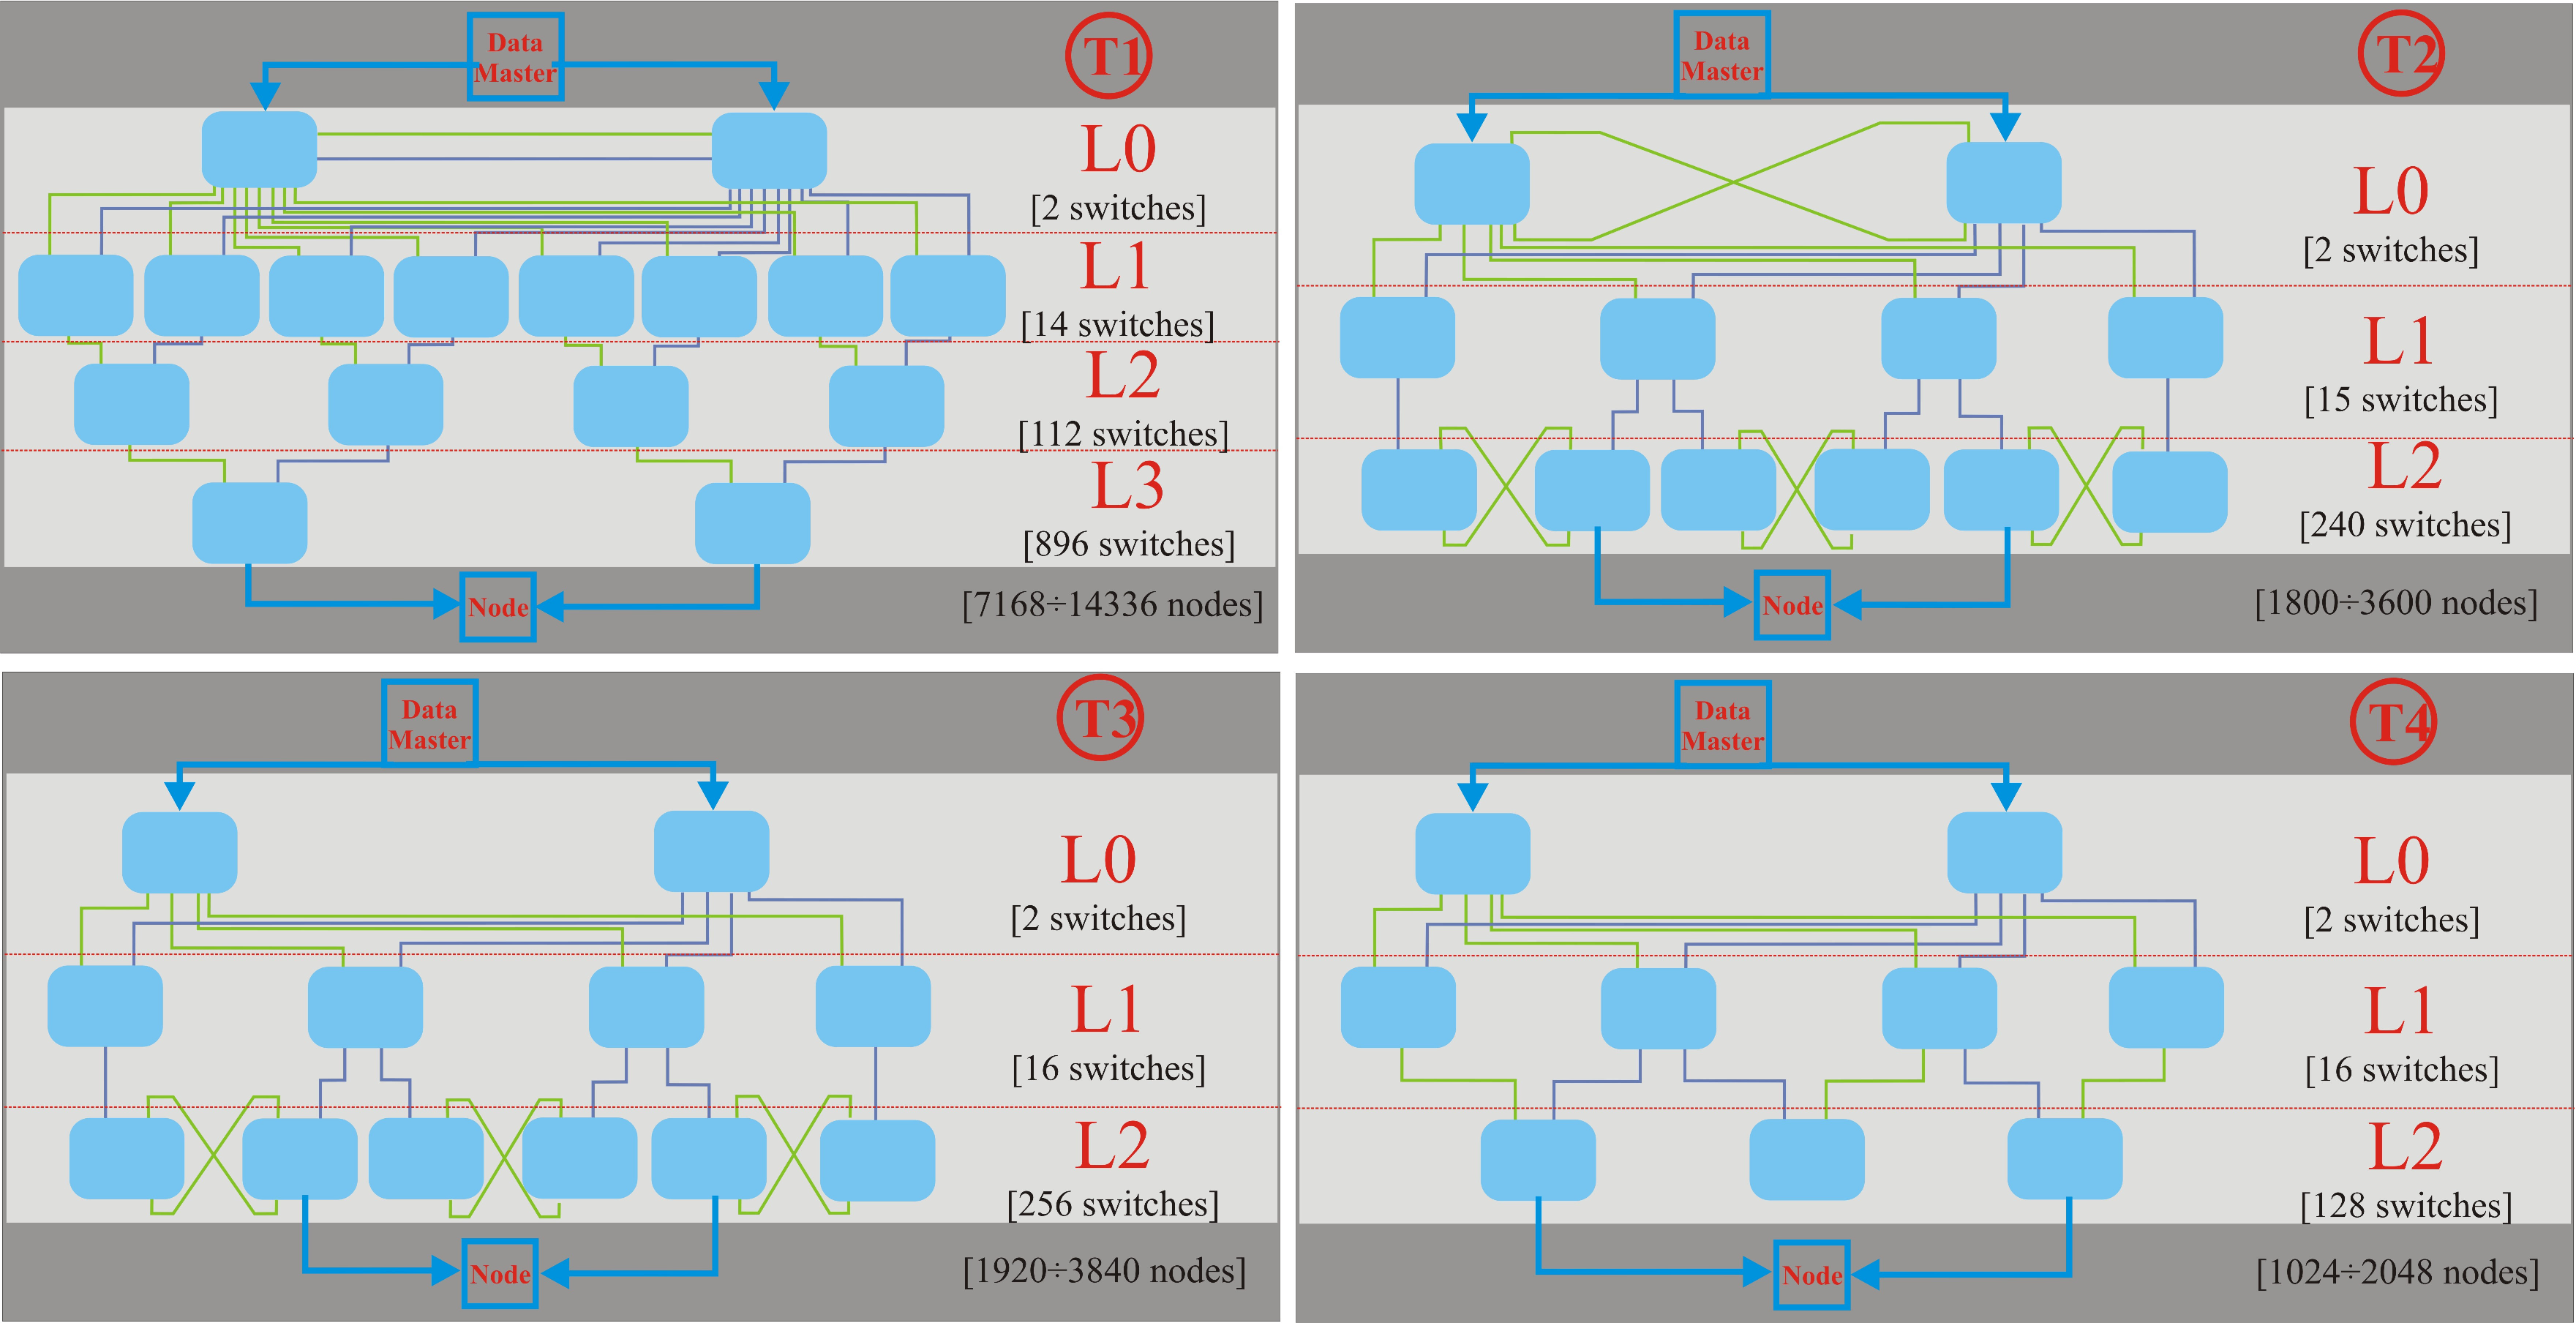
\includegraphics[scale=0.25]{../../../../figures/robustness/fullyRedundantTopologies.ps}
	\captionof{figure}{Topology examples with double redundancy.}
	\label{fig:fullyRedundantTopologies}
\end{center}

The number (probability) which is of the most interest in terms of WR Network
reliability, is the WR Network failure probability (k-terminal reliability),
which is the probability that at least one node (out of all) does not receive
messages ($P_{f\_Network}$). Unfortunately, precise estimation of
$P_{f\_Network}$ has not been obtained yet. However, it is clear that the number
is in the range of:
\begin{equation}
       P_f < P_{f\_Network} < nodes_number * P_f
\end{equation}

Table~\ref{tab:2000nodesReliability} presents rough estimations of WR Network
failure probability ($P_{f\_Network}$) for three considered topologies
($MTBF_{Switch}$= 200 000 [h]). However, to meet the requirement of $\approx
2000$ nodes, the topologies are of the type M-inputs/N-outputs where
$M \geq N$ (see also Table~\ref{tab:2000nodes3topologies}).

\begin{table}[ht]
\caption{Comparison of topologies with different level of redundancy,
M-inputs/N-outputs ($M \geq N$) and $\approx 2000$ nodes.}
\centering
\begin{tabular}{|p{4cm}|p{2cm}|p{2cm}|p{2.5cm}|p{2.5cm}|}        \hline
& \textbf{WRS Number} &
\textbf{Nodes MAX Number} &  
\multicolumn{2}{|p{5cm}|}{\textbf{$MTBF_{Switch}$=  20 000[h] }} \\
Topology & & & $P_f$ & MTBF[h]  \\ \hline
%1   &   3   &  14336  &   r1   &   r2   &   r3   &   r4   &   r5    \\ \hline

No-redundant &  127 &  2048  
& $ 2.08*10^{-3}$  & $ 5.77*10^{3}$
 \\ \hline

Double-redundancy &  292 &  2048  
& $ 4.71*10^{-7}$  &  $ 2.55*10^{7}$
   \\ \hline

Triple-redundancy &  495  &     
& $ 3.06*10^{-11}$  &  $ 4.08*10^{11}$
  \\ \hline
\end{tabular}
\label{tab:2000nodesReliability}
\end{table}

\subsection{Future enhancements}

The limitation which excludes ring topology from consideration is very
expensive. Ring topology might greatly limit the number of elements (switches
and links) preserving the level of high reliability. Additionally, ring topology
is a preferred choice in the industry. That is why, it needs to be considered
whether the current hardware limitation could be overcome to allow ring
topologies in the future.

\vspace{0.25cm}
